\documentclass[tikz,border=4pt]{standalone}
\usepackage[T1]{fontenc}
\usepackage{newtxtext,newtxmath}
\usetikzlibrary{arrows.meta,positioning,calc}
\definecolor{ink}{HTML}{203B50}
\definecolor{bluefill}{HTML}{EFF4F8}
\definecolor{teal}{HTML}{236D71}
\definecolor{tealfill}{HTML}{EFF7F5}
\definecolor{gray}{HTML}{646B72}
\begin{document}
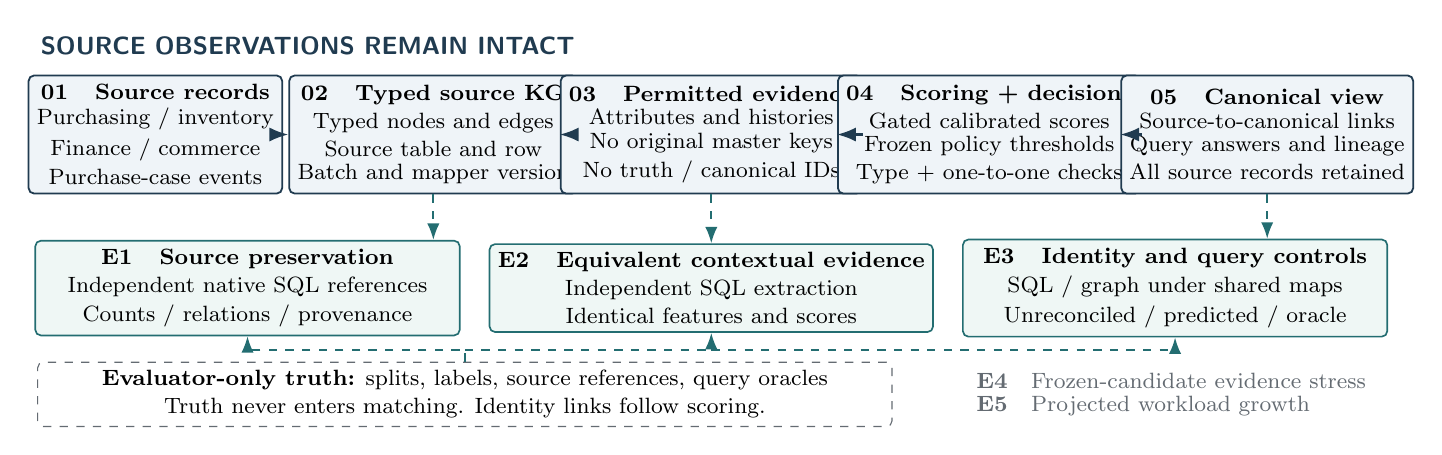
\begin{tikzpicture}[font=\fontsize{8.1}{10.6}\selectfont,>=Latex,
 stage/.style={draw=ink,line width=.65pt,rounded corners=2pt,fill=bluefill,align=center,minimum width=3.18cm,minimum height=1.50cm,inner sep=3pt},
 control/.style={draw=teal,line width=.6pt,rounded corners=2pt,fill=tealfill,align=center,minimum width=5.39cm,minimum height=1.05cm,inner sep=3pt},
 flow/.style={->,line width=.85pt,draw=ink},
 check/.style={->,dashed,line width=.65pt,draw=teal}]
\node[anchor=west,font=\sffamily\bfseries\fontsize{9}{11}\selectfont,text=ink] at (-.03,1.13) {SOURCE OBSERVATIONS REMAIN INTACT};
\node[stage] (s1) at (1.55,0) {\shortstack{\textbf{01\quad Source records}\\Purchasing / inventory\\Finance / commerce\\Purchase-case events}};
\node[stage] (s2) at (5.08,0) {\shortstack{\textbf{02\quad Typed source KG}\\Typed nodes and edges\\Source table and row\\Batch and mapper version}};
\node[stage] (s3) at (8.61,0) {\shortstack{\textbf{03\quad Permitted evidence}\\Attributes and histories\\No original master keys\\No truth / canonical IDs}};
\node[stage] (s4) at (12.14,0) {\shortstack{\textbf{04\quad Scoring + decisions}\\Gated calibrated scores\\Frozen policy thresholds\\Type + one-to-one checks}};
\node[stage] (s5) at (15.67,0) {\shortstack{\textbf{05\quad Canonical view}\\Source-to-canonical links\\Query answers and lineage\\All source records retained}};
\foreach \a/\b in {s1/s2,s2/s3,s3/s4,s4/s5}{\draw[flow] (\a.east)--(\b.west);}
\node[control] (c1) at (2.72,-1.95) {\shortstack{\textbf{E1\quad Source preservation}\\Independent native SQL references\\Counts / relations / provenance}};
\node[control] (c2) at (8.61,-1.95) {\shortstack{\textbf{E2\quad Equivalent contextual evidence}\\Independent SQL extraction\\Identical features and scores}};
\node[control] (c3) at (14.50,-1.95) {\shortstack{\textbf{E3\quad Identity and query controls}\\SQL / graph under shared maps\\Unreconciled / predicted / oracle}};
\draw[check] (s2.south)--(s2.south |- c1.north);
\draw[check] (s3.south)--(c2.north);
\draw[check] (s5.south)--(s5.south |- c3.north);
\node[draw=gray,dashed,rounded corners=2pt,align=center,fill=white,minimum width=10.85cm,minimum height=.72cm,inner sep=3pt] (truth) at (5.48,-3.30) {\shortstack{\textbf{Evaluator-only truth:} splits, labels, source references, query oracles\\Truth never enters matching. Identity links follow scoring.}};
\node[align=left,text=gray,inner sep=0pt] at (14.45,-3.30) {\shortstack[l]{\textbf{E4}\quad Frozen-candidate evidence stress\\\textbf{E5}\quad Projected workload growth}};
\draw[check] (truth.north) -- (5.48,-2.74) -- (2.72,-2.74) -- (c1.south);
\draw[check] (5.48,-2.74) -- (8.61,-2.74) -- (c2.south);
\draw[check] (8.61,-2.74) -- (14.50,-2.74) -- (c3.south);
\end{tikzpicture}
\end{document}
